\chapter{Capgemini à Rennes}
\section{Fiche d'identité}
\begin{description}
  \item[Locaux] : Le Spiréa - Zone des champs Blancs - Rennes
  \item[Année de construction] : 2012
  \item[Surface] : 9 850 m$^2$
  \item[Effectif en 2014] : 858
\end{description}
\begin{figure}[h]
  \captionbox{Le Spiréa à Rennes\label{fig:dummy}}{
    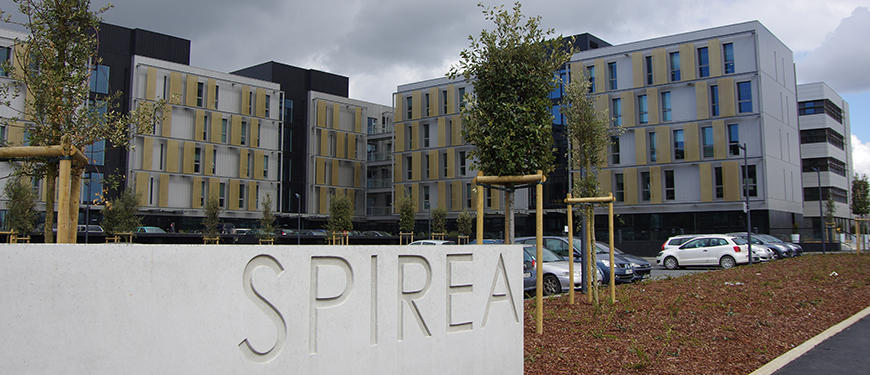
\includegraphics[width=15cm]{images/spirea.jpg}
  }
\end{figure}
\newpage
\section{Secteurs d'activités}
Le site de Rennes est divisé en 4 secteurs :
\begin{enumerate}
\item Aérospatiale et Défense
\item \textbf{ADM\footnote{Application Development and Maintenance} Center}
\item Services
\item Communications et EU\\
\end{enumerate}

\begin{colbox}{{HTML}{C7FF99}}{}
  Mon stage c'est déroulé dans la division ADM Center, sous-division ORANGE.\\
  Dirigé par Monsieur \textsc{Jean-Louis Hamon}
  cette sous-division s'occupe de la maintenance et de l'évolution d'applications logicielles du client ORANGE.
\end{colbox}

\section{Le centre de service TMA OSS}

La sous-division est gérée en plusieurs centre de services dont le service TMA OSS\footnote{Tierce Maintenance des Applications OSS d’Orange}.
Dirigé par Monsieur \textsc{Arnault Bellina} ce centre s'occupe de la maintenance des applications orientées réseau pour le client Orange.
Elle répond à diverses missions :

\begin{enumerate}
\item Développement d'évolutions
\item Soutien et maintenance
\item Audit et architecture
\item Assistance\\
\end{enumerate}

La TMA OSS gère 60 applications réparties sur 4 domaines différents :

\begin{enumerate}
\item \textbf{SIG\footnote{Système d’information géographique }}
\item Déploiement et interventions
\item Supervision QoS\footnote{Quality of Service}
\item RTG+\footnote{Ready-To-Go+} Supervision\\
\end{enumerate}

\section{Le domaine de compétence SIG}
\textsc{
Un système d’Information Géographique est un outil informatique permettant de représenter et d’analyser toutes les choses qui existent sur terre ainsi que tous les événements qui s’y produisent.
}\\\\
Les SIG offrent toutes les possibilités des bases de données (telles que requêtes et analyses statistiques) et ce, au travers d’une visualisation unique et d’analyse géographique propres aux cartes.
\\Ces capacités spécifiques font du SIG un outil unique, accessible à un public très large et s’adressant à une très grande variété d’applications.
Les enjeux majeurs auxquels nous avons à faire face aujourd’hui (environnement, démographie, santé publique…) ont tous un lien étroit avec la géographie.
De nombreux autres domaines tels que la recherche et le développement de nouveaux marchés, l’étude d’impact d’une construction, l’organisation du territoire, la gestion de réseaux, le suivi en temps réel de véhicules, la protection civile… sont aussi directement concernés par la puissance des SIG pour créer des cartes, pour intégrer tout type d’information, pour mieux visualiser les différents scénarios, pour mieux présenter les idées et pour mieux appréhender l’étendue des solutions possibles.
\\Les SIG sont utilisés par tous ; collectivités territoriales, secteur public, entreprise, écoles, administrations, états utilisent les Systèmes d’Informations Géographique (SIG). La création de cartes et l’analyse géographique ne sont pas des procédés nouveaux, mais les SIG procurent une plus grande vitesse et proposent des outils sans cesse innovant dans l’analyse, la compréhension et la résolution des problèmes.
\\L’avènement des SIG a également permis un accès à l’information à un public beaucoup plus large.
\\\\
Aujourd’hui, les SIG représentent un marché de plusieurs milliards d'euros dans le monde et emploient plusieurs centaines de milliers de personnes.
\begin{flushright}
\textit{source : Esri France}
\end{flushright}
\newpage
Lorsqu'on manipule des données géographique ont a besoin de les représenter correctement sur une carte, et pour cela il existe des normes, c'est ce qu'on appel la géodésie.

\begin{colbox}{{HTML}{A3E8FF}}{La géodésie\\}
  La géodésie est la science qui étudie les dimensions et la forme de la Terre, ainsi que son champ de pesanteur. Son objectif principal est d’élaborer des systèmes de référence terrestres auxquels tout utilisateur ou créateur de données géoréférencées peut accéder par l’intermédiaire de réseaux.
  \begin{flushright}
  \textit{source : IGN (Institut Nationale de l'information Géographique)}
  \end{flushright}
\end{colbox}
